\documentclass{article}
\usepackage{amsmath}
\usepackage{amsfonts}
\usepackage[utf8]{inputenc}
\usepackage[left=2.75cm,right=2.75cm,top=2.5cm,bottom=2.5cm]{geometry}
\usepackage{amssymb}
\usepackage{amsthm}
\usepackage{graphicx}
\usepackage{hyperref}
\numberwithin{equation}{section} 

\title{InverseMethod}
\author{Michi RAKOTONARIVO }
\date{January 2018}

\begin{document}

\maketitle

The aim of the data assimilation is to combine measured observations $y_k$ with the augmented model prediction $w_k^b$ to produce an update augmented model. This optimal estimate is called the analysis and denoted $w_k^a$. Hybrid variational method combined two methods: Extended Kalman filter and 3D Var.

\section{3D var}
The 3D var method is based on maximum a posteriori estimate approach and derives the analysis by seeking a state that minimizes a cost function $J$ measuring the misfit between the model state $w_k$ and the background state $w_a^b$ and the observation $y_k$
We define  the cost function as the following way:
\begin{equation}
    J(w_k) = (w_k - w_k^b)^T B_k^{-1} (w_k - w_k^b) + (y_k - \tilde h_k (w_k)) ^T R_k^{-1} (y_k - \tilde h (w_k)) 
\label{costFunc}
\end{equation}
Where $b_k$ and $R_k$ are the covariance matrices of the background and observation errors. \\
The solution for the analysis can be written explicitly as 
\begin{equation}
    w_k^a = w_k^b + K_k (y_k - \tilde H w_k^b)
\label{sol3D}
\end{equation}
The gain matrix is given by
\begin{equation}
    K_k =  B_k \tilde H_k^T(  \tilde H_k B_k \tilde H_k^T + R_k)^{-1}
\label{matrixGain3D}
\end{equation}


The 3D Var methods finds the analysis $w_k^a$ numerically using a gradient descent algorithm to iterate to minimize the solution.
The crucial difference between standard 3D Var and other schemes such as 4D Var and the Kalman filter is that the error covariance matrices are not evolved. The background error covariance matrix has a fundamental impact on the quality of the analysis.
%---------------------------------------------------------
\section{Extended Kalman filter(EKF)}  
With Extended Kalman filter, the state forecast is made using the full non-linear model.
For the state forecast, we have 
\begin{equation}
w_{k+1}^f = \tilde{f} (w_k^a, p_k^a)
\label{EKFfor}
\end{equation}
with $\tilde{f} $is the tangent of non-linear model forecast operator 
~~\\
The error covariance forecast is given by 
\begin{equation}
P_{k+1}^f = F_k P_k^a F_k^T
\label{CovEKF}
\end{equation}

where 
\begin{equation}
F_k = \big|_{w_k^a} \frac{\partial \tilde{f} }{ \partial w } = 
\begin{pmatrix}
\frac{\partial f(z,p)}{\partial w } & \frac{\partial f(z,p)}{ \partial p}\\
0 & I 
\end{pmatrix}  \big|_{{z_k^a},{ p_k^a}}
\label{EKFF}
\end{equation}

~~\\
The gain matrix is expressed as the following way
\begin{equation}
K_{k+1} = P_{k+1}^f H_{k+1}^T (H_{k+1} P_{k+1}^f H_{k+1}^T + R_{k+1}) ^{-1}
\end{equation}
where  $H_k = \big|_{w_k^a} \frac{\partial \tilde{h_k} }{ \partial w } = 
\begin{pmatrix}
\frac{\partial h_k(z,p)}{\partial w } & \frac{\partial h_k(z,p)}{ \partial p}\\
0 & I 
\end{pmatrix}  \big|_{{z_k^a},{ p_k^a}}$

~~\\
The analysis $w_{k+1}^a$ can be written as 
\begin{equation}
    w_{k+1}^a = w_{k+1}^f + K_{k+1} (y_{k+1} - H_{k+1} w_{k+1}^f)
\end{equation}
And finally, the analysis error covariance :
\begin{equation}
    P_{k+1}^a = (I - K_{k+1} H_{k+1} ) P_{k+1}^f
\end{equation}
The Extended Kalman method is computationally much costlier than 3D Var.  

%---------------------------------------------------------
\section{Hybrid approach}
Motivated by a desire of a low cost, uncomplicated alternative is to combined ideas from 3D Var and EKF to produce a new hybrid assimilation scheme. A simplified version of EKF forecast will be used to estimate parameters forecast error covariances, which will be combined with static approximation of the state background error covariances.

\subsection{Forecast step}
As mentioned before, for this section, we will use a simplified version of EKF. We can partition the forecast error covariance matrix  (\ref{CovEKF}) as follows
\begin{equation}
    P_k^f = 
\begin{pmatrix}
P_{xx_k}^f  & P_{xp_k}^f \\
(P_{xx_k}^f)^T &  P_{pp_k}^f 
\end{pmatrix}  
\end{equation}
where $P_{xx_k}^f $  and $P_{pp_k}^f $ are the forecast covariance matrix for the state $x_k$ at time $t_k$ and the parameter vector $p_k$. $P_{xp_k}^f $ is the covariance matrix for the cross relation between the forecast errors in the state and the parameter vectors \\
Using the EKF equations (\ref{EKFfor} , \ref{EKFF}), the analysis error covariance matrix is given by
\begin{equation}
    P_k^a = 
\begin{pmatrix}
P_{xx_k}^a & P_{xp_k}^a \\
(P_{xx_k}^a)^T &  P_{pp_k}^a
\end{pmatrix}  
\end{equation}
And if we denote $M_k = \frac{\partial f(x,p) }{ \partial z} \big|_{x_k^a, p_k^a} $ and $N_k = \frac{\partial f(x,p)}{  \partial p } \big|_{x_k^a, p_k^a}$, then we can write 
\begin{equation}
    F_k = 
\begin{pmatrix}
M_k & N_k \\
 0  & I
\end{pmatrix}  
\end{equation}
So, the error covariance forecast (\ref{EKFfor} ) is then expressed as
\begin{equation}
    P_{k+1}^f =  
\begin{pmatrix}
M_k & N_k \\
 0  & I
\end{pmatrix}
\begin{pmatrix}
P_{xx_k}^a & P_{xp_k}^a \\
(P_{xx_k}^a)^T &  P_{pp_k}^a
\end{pmatrix}
\begin{pmatrix}
M_k^T & 0 \\
 N_k^T & I
\end{pmatrix}
\end{equation}
Then, we substitute the state forecast error covariance matrix $P_{xx_k}^f $ with a standard 3D Var fixed approximation. And we assumed that the parameter error covariance matrix is also fixed, 
\begin{center}
    $P_{xx_k}^f =  B_{xx}$ ; $P_{pp_k}^f = B_{pp}$ for all k.
\end{center} 
So the forecast error covariance matrix is given by
\begin{equation}
    B_{k+1} = 
\begin{pmatrix}
B_{xx} & N_k B_{pp} \\
 B_{pp}N_k^T & B_{pp}
\end{pmatrix} 
\label{CovHyb}
\end{equation}

\subsection{Analysis step}
The analysis $w_k^a$ is found by substituting the matrix (\ref{CovHyb}) into the 3D Var cost function (\ref{costFunc}) and minimizing. The minimum is founding numerically using a gradient descent method. \\
The gain matrix (\ref{matrixGain3D}) can now written as 
\begin{equation}
K_k   =   B_k \tilde H_k^T(  \tilde H_k B_k \tilde H_k^T + R_k)^{-1} = \begin{pmatrix}
K_{x_k} \\
K_{p_k} 
\end{pmatrix} 
\label{GainHyb}
\end{equation}
The state and parameter analysis (\ref{sol3D}) are given by 
\begin{equation}
    x_k^a = x_k^b + K_{x_k} (y_k -  Hx_k^b) \\
\end{equation}
\begin{equation}
    p_k^a = p_k^b + K_{p_k} (y_k -  Hx_k^b)
\end{equation}
Then the gain matrices (\ref{GainHyb}) is expressed as 
\begin{equation}
K_{x_k} = B_{xx} H^T ( HB_{xx} H^T + R_k)^{-1}
\end{equation}
\begin{equation}
K_{p_k} = B_{pp} N_{k-1}^T ( HB_{xx} H^T + R_k)^{-1}
\end{equation}


%---------------------------------------------------------
\section{Applications}
To demonstrate this new hybrid method, there is a simple model which is a single parameter linear advection. It will be described.
%---------------------------------------------------------
\subsection{Linear advection}
%---------------------------------------------------------
\subsubsection{Model}
First, we consider the one-dimensional linear advection equation
\begin{equation}
\frac{\partial(u)}{\partial t} + a \frac{\partial u}{ \partial x} = 0  
\label{advEq}
\end{equation}
where a is the advection velocity.\\
The initial condition is 
\begin{equation}
u(x,0) = u_0(x)  , -\infty < x < \infty
\end{equation}
The solution of (\ref{advEq}) is simply 
\begin{equation}
u(x,t) = u(x_0,0) = u_0(x-at)
\label{solAdv}
\end{equation}
where $x_0 = x(0)$ and $x(t) = x_0 + at$. \\
We choose to solve (\ref{advEq}) for $a>0$ on a finite spatial domain $x \in [0,2]$ with the boundary condition 
\begin{center}
    u(t,0) = u(2,t) 
\end{center}
Using upwind scheme, we can express the solution as the following equation
\begin{equation}
u_j^{k+1} = u_j^k - a\frac{\Delta t} {\Delta x} ( u_j^k - u_{j-1}^k) 
\label{schemeNum}
\end{equation}
with the boundary condition $u_0^k = u_n^k$. \\
Denoting $\mu = \frac{\Delta t} {\Delta x} $, we can rewrite  (\ref{schemeNum})
\begin{equation}
u_j^{k+1} = (1- a\mu)  u_j^k - a\mu u_{j-1}^k 
\label{SimplNum}
\end{equation}


%---------------------------------------------------------
\subsubsection{Forecast step}
The \textbf{forecast model} (\ref{SimplNum}) can be expressed as the matrix system 
\begin{equation}
u_{k+1} = A  u_k 
\label{forecastAdv}
\end{equation}
where 
\[A = 
\begin{pmatrix}
(1-a\mu)  & 0&   &  &a\mu \\
 a\mu  & (1-a\mu) & 0&  &\cdots \\
 &\ddots & \ddots &\ddots & 0 \\
 0 & \cdots & 0 & \mu a & (1-a\mu)
\end{pmatrix}
\]
Since the velocity is constant, we have :
\begin{equation}
a_{k+1} = a_k 
\label{velocity}
\end{equation}


The \textbf{augmented system model} using (\ref{forecastAdv} and (\ref{velocity}) is given by 
\begin{equation}
w_{k+1} = f(w_k) = 
\begin{pmatrix}
A(a_k) & 0\\
0 & 1
\end{pmatrix} 
\begin{pmatrix}
u_k\\
a_k
\end{pmatrix} 
\label{MatrixA}
\end{equation}

%---------------------------------------------------------
\subsection{State-parameter covariance}
To compute the cross covariances between the errors in the model state $u$ ans the parameter $a$, we need to calculate the Jacobian of the forecast model with respect to the model parameters. This is given by 
\begin{center}
    $N_k  = \frac{\partial (A_k u_k)}{\partial a_k} \big|_{u_k^a, a_k^a}$
\end{center}

From (\ref{MatrixA}), we have
\begin{equation}
\frac{\partial A_k}{\partial a_k} = 
\begin{pmatrix}
-\mu  & 0& & \mu\\
\mu  & -\mu & 0 & \cdots \\
 & \ddots &\ddots &\ddots&0\ \\
 0 & \cdots & 0 & \mu & -\mu 
\end{pmatrix} 
\end{equation}
Then the matrix $N_j$ is given by
\begin{equation}
    N_j = \frac{\partial u_j^{k+1}}{\partial a_k} = -\mu ( u_j^k - u_{j-1}^k)
\label{N}
\end{equation}
Since, we have only a single unknown parameter, the parameter $p^b$ is scalar and 
\begin{equation}
    B_{pp} = \sigma_a^2
\label{Bpp}
\end{equation}
where $\sigma_a^2$ is the error variance.
Combining (\ref{N} and \ref{Bpp}), the cross variance between the parameter error $\epsilon_a$ and the element $j$ of the state background error $\epsilon_u $ at time $t_{k+1}$ is expressed as
\begin{equation}
    B_{up}^{k+1}(j)  = \sigma_a^2  \mu ( u_j^k - u_{j-1}^k)}
\end{equation}
%---------------------------------------------------------
\subsection{Results}
\subsubsection{Parameters}
In this example, we will take the following parameters:
\begin{itemize}
\item The true advection velocity a=0.5
\item initial parameter estimate $a_0 $is generated by adding Gaussian random noise with zero mean and variance $\sigma_a^2 = 0.1$
\item Observations are generated by sampling the analytic solution (\ref{solAdv}) on a regularly spaced grid and are assimilated at regular time intervals
\item The state background error $B_{xx}$ is kept fix
\item The parameter background matrix $B_{pp}$ is fixed as well.
\item The state-parameter cross variance matrix $B_{xp}$ is recalculated at each new assimilation time
\item And at the end of each assimilation cycle, the model parameters updated
\end{itemize}
To characterize the \textbf{state background errors}, we use the isotropic correlation function :
\begin{center}
    $b_{ij} = \sigma_b^2 \rho ^{|i-j} $
\end{center}
where element $b_{ij}$ defines covariance between components $i$ and $j$ of state background error vector $\epsilon_u = u^b - u^t$. \\
The \textbf{observation error covariance matrix} is expressed as 
$R_k = \sigma_0^2 I$ \\
The model is runt on the domain $x \in [0,2]$.
The true solution is shown in figure \ref{trueSol} \cite{HybridSequential}.
We adopt a 3D Var approach and minimize the cost function (\ref{costFunc}) iteratively using a quasi-Newton descent algorithm.

\begin{figure}[h]
    \begin{center}
    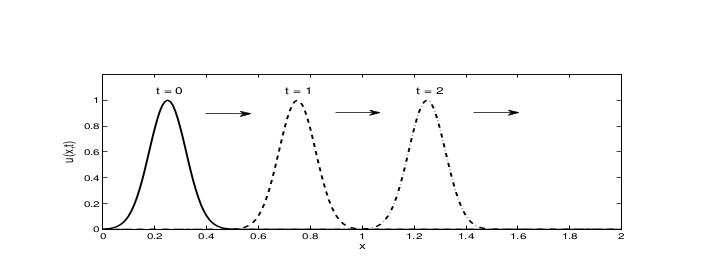
\includegraphics[width=15cm]{trueSolAdvection.png}
    \caption{Linear advection model: true solution $u(x, t)$}
    \label{trueSol}
    \end{center}
\end{figure}


\subsubsection{Perfect observations}
The value of the initial estimate $a_0$ is $a_0= 0.87116$. \\
As the name section indicates, the observations are perfects which means that no noise is adding in the observations.
The results is represented in the figure \ref{perfectObs} \cite{HybridSequential}.\\

\begin{figure}[h]
    \begin{center}
    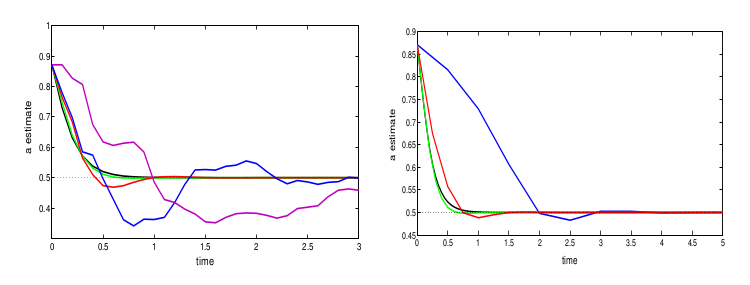
\includegraphics[width=9cm]{perfectObsAdvection.png}
    \caption{Perfect observations: parameter updates for initial estimate a = 0.87116.
(a) Varying the spatial frequency of observations: solid black line - observations at $2\Delta x$ intervals; solid green line -
observations at $5\Delta x$ intervals; solid red line - observations at $10\Delta x$ intervals; solid blue line - observations
at $25 \Delta x$ intervals; solid purple line - observations at $50\Delta x$ intervals. (b) Varying the temporal frequency
of observations: solid black line - observations every $5\Delta x$; solid green line - observations every $10\Delta x$; solid
red line - observations every$25\Delta t$; solid blue line - observations every $50\Delta t$.}
    \label{perfectObs}
    \end{center}
\end{figure}

\begin{itemize}
    

\item  Figure \ref{perfectObs} (a) shows the effect of varying the spatial frequency of observations for the initial estimate. Observations are assimilated every $10\Delta t$, with $\sigma_0^2 = 0.01$ and grid spacing between observations range from every $2\Delta x$ to every $25\Delta x$. The scheme performs extremely well.For observations taken every $2\Delta x$, $10\Delta x$ and $25\Delta x$ the scheme recovers the true value of a to a high level of accuracy. The quality of the state analysis is also high. To every 50 and 100 , the estimates take much longer to stabilise. With observations every $100\Delta x$ the $a$ estimate gets close to but never quite settles on the true value of $a$. 

\item  Figure \ref{perfectObs} (b), shows the effect of varying the temporal frequency of the observations for the same starting estimate $a_0$. Observations are taken every $5\Delta x$, and assimilated at intervals of $5\Delta t$, $10\Delta t$, $25\Delta t$ and $50\Delta t$. The results are similar to the previous experiment there is a differnce when the time when the time between successive assimilations is increased from every $5\Delta t$ to $10\Delta t$ to $25\Delta t$. For observations every $50\Delta t$ the a estimate takes slightly longer to converge. If this period is doubled again to $100\Delta t$ the scheme completely fails to recover $a$.
\end{itemize}

\subsubsection{Noisy observations}
In this section, we add noise in the observations. The noise is defined as Gaussian with mean zero and variance $\sigma_a^2$. And the results are represented in the figure \ref{noisyObs} \cite{HybridSequential}.
\begin{figure}[h]
    \begin{center}
    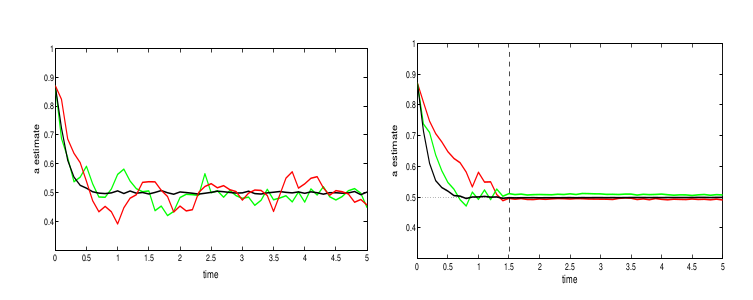
\includegraphics[width=9cm]{noisyObs.png}
    \caption{Imperfect observations: parameter updates for initial estimate $a = 0.87116$ (a) unaveraged estimates, and (b) time averaged estimates: solid black line $\sigma_0^2 = 0.001$; solid green line $\sigma_0^2 = 0.01$; solid red line $\sigma_0^2= 0.1$}
    \label{noisyObs}
    \end{center}
\end{figure}

\begin{itemize}
\item Figure \ref{noisyObs} (a) shows the parameter a estimates produced for error variance increasing from $\sigma_a^2=0.001$ to $\sigma_a^2=0.1$
The results is that when the observations are noisy, then resulting analysis and estimate parameters are also noisy. The amplitude of oscillations in $a$ increase as $\sigma_a^2$ is increased. When the $\sigma_a^2$, the state analysis is particularly messy. The oscillations are approximately centered around a true value $a$


\item In figure \ref{noisyObs} (b),the same experience above is repeated but with the $a$ estimates being averaged over a moving time
window of 20 timesteps.

\end{itemize}
%---------------------------------------------------------




%---------------------------------------------------------
\section{Conclusion}
A key difficulty in the construction of a data assimilation algorithm is specification of the background error covariances. These covariances play an important role in the filtering and spreading of observational
data and have a direct influence on the quality of the analysis

As the results obtained showed, the scheme performed well in all of the three
cases considered and was successful in recovering the parameter values we had specified to a good level of accuracy, even when the observational data were noisy. This had a positive impact on the skill of the forecast model and enabled more accurate predictions of the true model state.


%\section*{Bibliographie}
\addcontentsline{toc}{section}{Bibliography}
\bibliographystyle{plain}
\nocite{*}
\bibliography{biblio}
\end{document} 

